\documentclass[showkeys,aps,prb,prepreint,amssymb, amsmath,nobibnotes]{article}
\usepackage{bm,setspace}
\usepackage{graphicx,graphics,booktabs}
\usepackage[a4paper,margin=2cm]{geometry}
\newlength{\dhatheight}
\onehalfspacing

\title{How to analyse NMR relaxation data. If dynamics are important, how do you measure them?}
\author{Andrew Baldwin, Ollie Crooks}
\begin{document}
\maketitle

\abstract{It follows from the strength of individual intermolecular forces holding a protein together being on the order of $k_bT$ that proteins are dynamic. But how can we experimentally determine how proteins move? Relaxation rates determined by NMR spectroscopy are strongly coloured by both local and global motions. It remains challenging to extract from these a coherent and quantitative picture of the underlying molecular dynamics. We will work through the state of the art, and then replace it with something far better. Precisely what that is, TBD. But it's going to be great.
}

  \section{Introduction}

  Nuclear spins inside a protein have a complex and turbulent environment, magnetically speaking. Individual nuclear spins interact in various ways and their fields couple. In an NMR spectrometer, we exploit the fact that the ensemble of molecules in our sample end up behaving as a single spin. We can then coherently manipulate all spins at once using RF pulses. This is truly remarkable - all spins in the sample, across Avogadro's number of molecules all rotate in perfect unison.

  This simply can't be done with optical spectroscopies. The reason we can get away with this is because the energy level differences for NMR are small, on the order of radio frequencies, a few MHz. This has the consequence that our spin state population differences are tiny, on the order of a few parts per million. So NMR as we practise it today can never be a single molecule technique. At these energy level differences, there are few mechanisms for the perturbed spins to return to thermal equilibrium. Normally in spectroscopy, the relaxation is dominated by spontaneous emission, which is quantitatively described by one of the Einstein coefficients. This rate goes with the difference in energy between the states raised to the 4th power. For NMR, this rate ends up being measured in units of universe lifetimes (with values greater than 1). So while this mechanism dominates almost all other spectroscopies, it does not cause appreciable relaxation in NMR experiments. It is remarkable then that for NMR, the major mechanism to return back to equilibrium is the second process identified by Einstein, stimulated emission, where transitions between spin states are triggered when a spin is exposed to a local field that matches the energy level difference.

  Where can such fields come from in solution? This happens after we've turned the pulses off, so we only have the static magnetic field strength and adjacent molecules to think about. The fun realisation is that the fields are generated by the underlying motion of molecules themselves. Take for example two nuclear spins in a molecule, say two protons. Classically these behave as bar magnets, and as a molecule undergoes rotational diffusion, the fields experienced at each site vary as the vector linking the position of the two spins varies. Diffusion is a Brownian processes, and so the fluctuations are random. However, we observe our spins in experiments for seconds, whereas rotational correlation times for proteins are nano-second. So any individual spin at certain points in its trajectory will certainly undergo motions that leads to the coherent development of a magnetic field with a characteristic frequency. When these randomly generated fields end up matching a relevant energy level difference in the spin system, then we have a path open for a transition, and a route to get back to equilibrium. The probability of generating such fields from random motion is low, and so we have the non-intuitive idea that nano-second motions (and faster) are the cause of relaxation rates on the seconds time scale. 
 
  Relaxation in NMR then is caused entirely by the local jigglings and wigglings of atoms, and so is highly sensitive to local motion. In what follows we will state some results for relaxation rates that are both easy to measure by NMR, and provide a relatively unambiguous route by which they can be modelled in terms of local groups (a single NH pair) without the need to worry about the rest of the molecule. We sketch out the theory that links local motion to the relaxation rates and go through the methods conventionally used to link relaxation rates to underlying molecular motions. These bring with them some truly horrendous assumptions, such as local motion at one residue in a protein being entirely independent of local fluctuations occurring at an adjacent residue. Which is utterly unphysical and has really held NMR back from being a true `go-to' method to provide immediate quantitative pictures of underlying molecular dynamics derived from experiments.

  By recasting the problem in terms of the need to reduce the dimensionality of the various timescales and revisiting how we analyse the data, we aim here to produce a method to generate a coherent description of underlying molecule motions experienced by proteins. Given we can download datasets for hundreds of proteins, we can make a big splash with this work.
  
 
 
  \section{NMR relaxation rates}

  If we consider a single isolated spin half, then it turns out that we need to describe it using a three element basis in order to describe everything that it can do. This has an excellent physical picture (the Bloch sphere), with magnetisation aligned on either the $x$, $y$ or $z$ axes, described by the quantum mechanical operators $I_x$, $I_y$ and $I_z$. When we consider coupled spins, we have to use a basis that includes all combinations of these axes for the two spins, leading to the requirement of a basis that has 15 operators constructed via outer products, such as $I_xS_x$, $I_zS_x$ and so on. We can calculate the rate at which the different states relax using Redfield theory. This reveals that each state not only has an auto-relaxation (which looks simply like spontaneous decay), but there are also relaxation rates that lead to cross relaxation between states. The most commonly encountered example of this is the nuclear Overhauser effect or NOE, which is widely exploited in chemistry and biochemistry. This is a relaxation process that couples operators such as $I_z$ and $S_z$, leading to transfer of information between them. Magnetisation can `jump' from the $I$ spin to the $S$ spin in a suitable experiment, in a manner that depends on how far apart the spins are. This effect is the basis of protein structure determination by NMR, allowing us to use this effect as a weak ruler to measure inter-spin distances, from which an atomic resolution structure can be calculated.

  This has an important consequence for determining protein dynamics by NMR. If magnetisation is jumping from one spin to another and running all over a protein, it becomes tremendously difficult to pin down and analyse. When performing a Redfield calculation, we need to identify all relevant interactions that can cause a spin to experience a randomly fluctuating time dependent field. In proteins, the strongest by a considerable margin is the proton-proton dipolar coupling. This is large because the strength goes with gyro-magnetic ratio ($\gamma$) to the power of 4, and $\gamma_H\approx 4 \gamma_C \approx -10 \gamma_N$. But also the effect goes with $\frac{1}{r^6}$ and protons are typically as close as it is possible to get within a protein. The proton-proton NOESY effect has dominated NMR protein structure elucidation for this reason. But when trying to neatly measure protein dynamics, we need to steer clear of proton-proton NOESYs, as to analyse these requires us to understand the spatial relationships between all protons in a protein and how this is buggering around over the entire molecule. For this we certainly need a structure.

  Conveniently, we can look at NH spin pairs in protein samples that have been enriched with $N^{15}$. The amide nitrogen amides are far from all other nitrogens. They have a covalent bond to an adjacent proton, cleverly named the amide proton (possessed by all residues in the protein other than prolines and the N-terminal residue). This single bond then should largely dominate the fields that lead to its relaxation. Of the 15 coherences we can easily generate from the NH spin pair, we first restrict our attention then to coherences that are localised on the nitrogen only. These are the relaxation rates associated with transverse nitrogen ($N_x$ or $N_y$, these have identical relaxation rates), the rate associated with longitudinal nitrogen ($N_z$), and the heteronuclear NOE rate where we determine the extent to which magnetisation can build up on the nitrogen from knocking the amide proton well out of equilibrium.

  There exist a host of other coherences we could inspect. States like $N_xH_z$ will cross relax among each other via the protons, and so again will be hard to study. We can generate so called `multiple quantum' coherences like $N_xH_x$. These should not suffer from cross relaxation and so we probably really should routinely measure these and add them to the dataset. This is not widely done and most the downloadable data we'll get will not have these.

  Other than the NH dipolar interaction, the next largest field experienced by a nitrogen is its `chemical shift anisotropy'.The chemical shift is caused by the static magnetic field causing ring currents in electron clouds. This can be well understood via the Biot-Savart law, where a moving particle with charge will experience a torque when placed in a magnetic field. These motions (we now have a moving charged particle) will generate a new magnetic field. This will compete with the static field (Len's law). This is a small effect in the big picture (on the order of parts per million) but is large enough that we can easily measure it.

  In solution NMR experiments, the `peaks' we see have a chemical shift measured in ppms, and we use these to routinely distinguish electronic environments within a molecule. The isotropic chemical shift is the shift you get from rotationally averaging all orientations of the molecule under study. In a real molecule, the distribution of bonding electrons is not isotropic. Take a sigma bond: these follow an inter-atom bond vector, and are not at all spherically distributed. This means that at any instance of time, the bond has some alignment with the static magnetic field, generating a field at each nucleus. When the molecule changes orientation, the fields change. And so this effect leads to a time dependent fluctuating field capable of causing relaxation, in a manner that gets stronger the more `anisotropic' the electron cloud. Amide bodes have additional $\pi$ electrons, which make this mechanism particularly relevant for analysing the relaxation of backbone $N^{15}$ nuclei, as the surrounding electron density is `lumpy'. Density functional theory does a terrific job of computing not just the chemical shift, but also its complete tensor, from which we can determine both the isotropic chemical shift (observed as the Central peak position in a spectrum), and also its anisotropic parts (which will contribute to relaxation).

  In the spirit of being completionist, the final interaction relevant for NMR is the quadrupolar interaction. This occurs only for nuclei with spin bigger than $\frac{1}{2}$. This makes life complicated and more often than not, we run away screaming from these, avoiding them like the plague.

  To analyse protein dynamics then, conventionally we measure the transverse and longitudinal relaxation rates of $N^{15}$, called $R_2$ and $R_1$ respectively because this is what the great Felix Bloch named them, and the heteronuclear NOE. From the perspective of the nitrogen, we need to worry a lot about the adjacent proton, as it is very close, and its dipolar field dominants relaxation. We also need to worry about nitrogen's chemical shift anisotropy (CSA). The orientation of these two interactions might not be co-linear, in a manner that will depend on the detailed local environment. We would like though to analyse data in a manner that doesn't require the structure to be known, to put in interaction constants that reflect the mean field. But things like variation in NH bond length due to hydrogen bonding, bond orientation changing the axis of the CSA tensor, and changing the chemical nature of adjacent residues will cause variations in the interaction strengths. We're going to largely hope that these fluctuations are small.
  
  Finally, we need to consider how specific motional models cause fluctuations in these fields and hence drive relaxation. If the fluctuations between two sites are truly random, there is no prospect of generating coherent fields and the motion is not capable of driving relaxation. Rotational tumbling is an interesting case because it keeps all bond vectors constant in principle, which fixes the strength of say the maximum strength of dipolar interaction (determined only by distance). This is very capable of generating high frequency fluctuations that have some probability of generating coherent fields that can cause relaxation. More generally any fluctuations that lead to coherent variation in fields can drive relaxation, which should extend to local `breathing' type motions, whose amplitudes and timescale will vary with residue.

  We are going to occasionally refer to to `chemical exchange' effects, which for proteins can be interpreted as the presence of additional micro and milli-second dynamics causing conformational changes in proteins. We can study these quantitatively to do things like understand enzyme mechanism. We collectively call these `slow' dynamics. The relaxation studies we are talking about here are for `fast' dynamics (ns timescale and quicker) for which chemical exchange effects lead to $R_2$ being bigger than we'd otherwise expect. We can independently quantify these effects experimentally should we need to, and this is the best way to access these types of motions, and to separate milli/micro second dynamics from nano/pico second dynamics.
  
  In a fast dynamics NMR study then, we try to separate global motion from local. Global motional parameters are restrained globally for all residues, and local ones can be, say, residue specific. As ever, if our model gives us a good fit, judged normally by a $\chi^2$, we can bring the machinery of Baye's into the game and use this to guide us. As we have flat priors the probability of a model and parameters explaining the data is proportional to $e^{\chi^2/2}$, which is very nicely explained in the text book Numerical Recipes in C. Adding more parameters into a model should all ways round lower the $\chi^2$ and so F-statistics can be employed to help guide our journey to ask if the probability that the reduction in $\chi^2$ in going from from a low complexity model (fewer parameters), to high complexity models (more parameters) is significant. The path is a always a wonky one and it would be nice if we can automate this type of analysis to generate a coherent description of molecular dynamics.

  In the next sections we state expressions for the relaxation rates commonly used and values for the fields. The rates are plotted versus rotational correlation time to help give a field for how they vary. We then look at how different motional models give rise to different forms of correlation functions, from which a `spectral density function' can be computed, that ultimately parameterises the relaxation rates. Our goal is to find a minimally complex picture of the dynamics that lets us understand both local and global motions of the molecule we're analysing. We also want this picture to provide physical insight so we can quantitatively analyse the underlying molecular motions.
  

  \subsection{Specific relaxation rates used for backbone dynamics}

\begin{figure}
  \center
  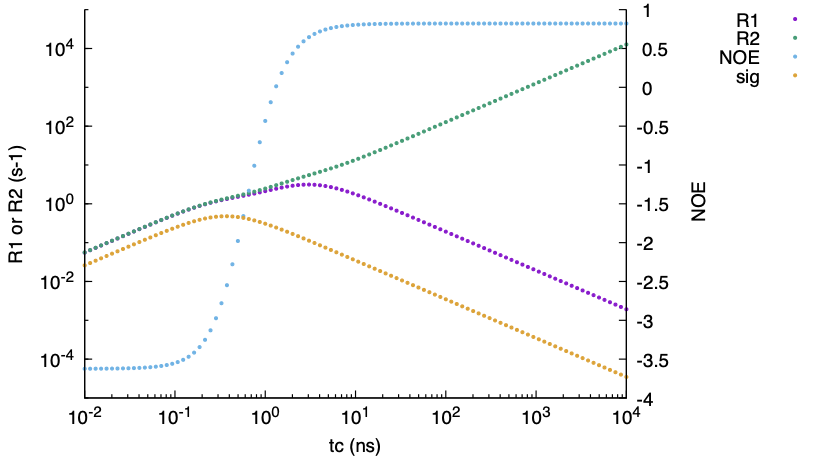
\includegraphics[width=0.49\textwidth]{mathsFigs/RelaxationRatesCorr}
  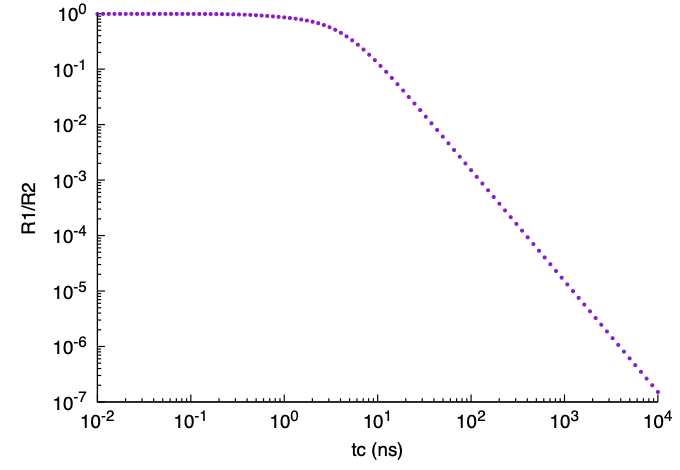
\includegraphics[width=0.49\textwidth]{mathsFigs/R1R2}
\caption{Left: Plot of $R_1$, $R_2$, $\sigma$ and the NOE as a function of correlation time, for rigid bodies undergoing isotropic tumbling. The two regimes at low and high correlation time can be clearly resolved. $R_2$ just keeps getting bigger, whereas $R_1$ and $\sigma$ have a maximum. The NOE depends on the ratio of $\sigma$ and $R_1$, and has a convenient sigmoidal form, rendering it especially sensitive to local motion. On the right is a plot of $R_1/R_2$ versus correlation time, which when we only have dipolar interactions, follows equation \ref{eqAll}. }
\label{RatesSimfig} 
\end{figure}


 
Details of a Redfield theory computation can be found in the RelCalc paper. But to state the result, the three relevant relaxation rates here assuming NH dipolar coupling, isotropic global tumbling and chemical shift anisotropy are  

\begin{equation}
    \left(\begin{array}{c} R_1 \\R_2 \\ \sigma \end{array}\right)
    =
  \frac{1}{5} \left(\frac{1}{4}d^2 
   \left(\begin{array}{ccccc}
     0 & 0 & 6 & 2 & 12 \\
     4 & 6 & 3 & 1 & 6 \\
     0 & 0 & 0 &-2 & 12 \\
   \end{array}\right)
   +
   C_A^2
      \left(\begin{array}{ccccc}
     0 & 0 & 1 & 0 & 0 \\
     4 & 0 & 3 & 0 & 0 \\
     0 & 0 & 0 & 0 & 0 \\
   \end{array}\right)
   \right)
   \left(\begin{array}{c} J(0) \\ J(\omega_H)  \\J(\omega_N) \\  J(\omega_N-\omega_H) \\ J(\omega_N+\omega_H) \end{array}\right)
   \label{eqAll}
  \end{equation}

where the spectra density function is $J(\omega)$, and the dipolar interaction constant $d=\frac{\mu_0 \hbar \gamma_H\gamma_N}{4\pi r^3}$. For an HN spin pair undergoing dipolar coupling, a commonly used bond distance is 1.022 \AA. The CSA interaction constant is $C_A=\frac{1}{3}\gamma_NB_0(\delta_{zz}-\delta_{yy})$ where the $\delta$ components are principal components from the chemical shift interaction tensor, which takes a value of -160 ppm for a typical NH pair. The chemical shift anisotropy should be placed at an arbitrary angle with respect to the dipolar interaction, but under the assumption of isotropic tumbling, because there is no cross-correlation between the two effects, both dipolar and CSA mechanisms provided independent contributions to the rates. Things are not so simple when we start to include non-isotropic global tumbling, but RelCalc provides a great tool to handle this complexity. Rates are shown versus the rotational correlation time $\tau_c$ in figure \ref{RatesSimfig} showing their regimes assuming isotropic tumbling.

Each rate samples 5 different frequencies from the spectral density function, but with different weightings. These frequencies arise because they are associated with specific transitions that occur at those specific values. $R_1$ describes the return to thermal equilibrium via population changes. This requires us to strongly re-assert the population difference between $\alpha$ and $\beta$ spin states, to get back to a Boltzmann distribution (thermal equilibrium). This is driven by transitions on a frequency of $\omega_N$, which is the energy level difference between the two states. The spectral density of generating this frequency is $J(\omega_N)$ and so this is the leading term for $R_1$.

$R_2$ is slightly more complex. Here, fluctuations cause a loss of coherent oscillation. Physically this can be understood by thinking of the coherent oscillation of synchronised spins aligned macroscopically over the sample (the NMR signal) getting out of phase because of small fluctuations, an entropic rather than an enthalpic effect. This has no energy associated with it, and so is dominated by the zero frequency term $J(0)$. This doesn't describe a transition, and can be thought of as the loss of coherence occurring just because of fluctuations cause by Langevin dynamics at zero energy. This is the loss of coherence.

The chemical shift anisotropy term samples only the frequencies $J(0)$ and $J(\omega_N)$. Because this mechanism is restricted to the nitrogen, there is no appearance of proton fields. 

The steady state heteronuclear NOE measurement is given by

\begin{equation}
  \mathrm{NOE}=1+ \frac{\gamma_H}{\gamma_N}\frac{\sigma}{R_1}.
  \label{eqNOE}
\end{equation}

Here, we do an experiment where we detect nitrogen magnetisation, when the amide proton is at thermal equilibrium. Then we do a second experiment where we first smack the living crap out of the amide proton, and measure the difference. In the second case, we get cross relaxation between the nitrogen and the proton, so the difference is driven by cross relaxation, which in this case is also normally called the nuclear Overhauser effect. In the most basic model, where we consider only isotropic tumbling as the source of the motion, then the spectral density function that plugs into the above model is
\begin{equation}
J_{\mathrm{RigidBody}}(\omega)=\frac{\tau}{1+\omega^2 \tau^2}
  \end{equation}

where $\tau$ is the rotational correlation time.

To get some insight into the various rates, we can see that this leads to two limiting regimes. The first is in the 'small molecule' limit, where $\tau \omega << 1$. Here, $J(\omega)\approx\tau$, and there is substantial (uniform) spectral density at all relevant frequencies. In this limit,

\begin{equation}
    \left(\begin{array}{c} R_1 \\R_2 \\ \sigma \end{array}\right)
    =
    d^2 \tau \left(\begin{array}{c} 1 \\ 1 \\ \frac{1}{2}  \end{array}\right)
  \end{equation}

Here, $R_1=R_2$ and $\mathrm{NOE} = 1+ \frac{\gamma_H}{\gamma_N}\frac{1}{2} = -4$ because $\frac{\gamma_H}{\gamma_N}\approx -10$. We see things tend to this limit at the C termini of ubiquitin and if we were looking at small molecules, this is what we would see. The opposite regime is the macromolecular limit, which we roughly hit for flexible regions in proteins. Here $\tau\omega >> 1 $. Then 

\begin{equation}
    \left(\begin{array}{c} R_1 \\R_2 \\ \sigma \end{array}\right)
    =
    \frac{1}{10}d^2
    \left(\begin{array}{c} J(\omega_N-\omega_H) \\ 2 \tau \\ - J(\omega_N-\omega_H) 
    \end{array}\right)
  \end{equation}

We can see that $R_2$ grows monotonically with $\tau$ for its entire range, though its growth is slower in the high molecule limit. The steady state NOE tends to $1$ in the big molecule limit because $R_1$ will get larger than $\sigma$ as $\tau$ grows, so this from -4 in the small molecule limit, to 1.

$R_1$ and $\sigma$ are a bit more interesting. In the small molecule limit, they both grow linearly with $\tau$, like $R_2$. In the large molecule limit though, they decrease in size as $J(\omega_N-\omega_H)$ and $J(\omega_N+\omega_H)$ both get smaller the larger $\tau$ gets. This leads to the emergence of an optima at an intermediate value of $\tau$, that occur roughly when $\omega_N\tau \approx 1$. 


\section{Correlation functions}

\begin{figure}
\center
  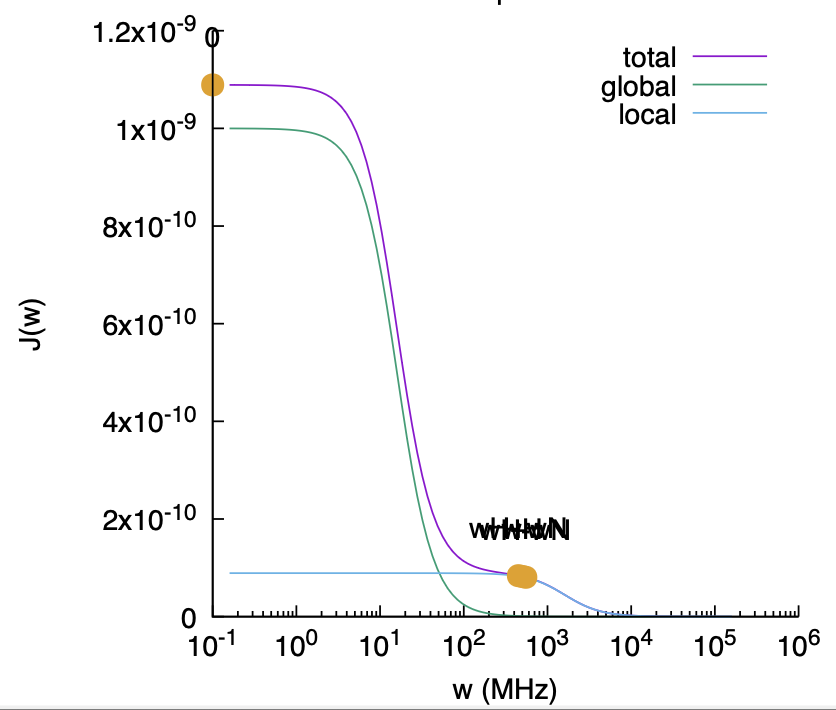
\includegraphics[width=0.5\textwidth]{mathsFigs/Jomega}
  \caption{The model free spectral density function with $\tau_c$ of 10 ns (reasonably big protein), $\tau_e$ for local fluctuations at 100 ps, and $S^2$ 0.1 (mostly local motion). The specific frequencies sampled by the measurements, $0$, $\omega_H$, $\omega_N$, $\omega_H+\omega_N$ and $\omega_H-\omega_N$ are indicated by orange points. The zero frequency point has been shifted for clarity. $J(0)$ is dominated by global motion, but this decays to zero quite quickly. The local motion largely dominates at higher frequencies. On a log plot, all of the non-zero frequencies are actually very close to each other, differing by a factor. We expect then that $R_2$ is mostly affected by global tumbling, whereas $R_1$ and $\sigma$, being derived from higher frequency transitions, are mostly affected by local.}
\label{Jfig}
\end{figure}


Before going on, look at the spectral density functions. Different motional models lead to different correlation functions, which in a very general case is built up of sums of independent motion and amplitudes, such that

\begin{equation}
  C_{\mathrm{General}}(\tau)= \sum_i  A_{i} e^{-\frac{\tau}{\tau_i}}+ \sum_{ij} A_{ij} e^{-\frac{\tau}{\tau_i}-\frac{\tau}{\tau_j}}+ \sum_{ijk}  A_{ijk} e^{-\frac{\tau}{\tau_i}-\frac{\tau}{\tau_j}-\frac{\tau}{\tau_k}} +...
  \end{equation}

where we consider motion on a range of timescales. The sum of all amplitudes $A$ is 1. The first sum describes a straight decay of independent processes. The second describes combined timescales, which could be local and global fluctuations, and so on. Lipari and Szabo's famous `model free' assumes two timescales where

\begin{equation}
  C_{\mathrm{modelFree}}(\tau)= S^2 e^{-\frac{\tau}{\tau_c}} + (1-S^2) e^{-\frac{\tau}{\tau_c}-\frac{\tau}{\tau_e}}
  \end{equation}

This says a spin is exposed to fluctuations because of global tumbling only, whose specific amplitude is $S^2$ where $S$ is an order parameter. It then says the spin is also exposed to fluctuations on a faster timescale, $\tau_e$, which combines with global tumbling causing relaxation on a more rapid timescale, obtained from taking the average of the reciprocals. We recover the rigid body tumbling correlation function by setting $S=1$, and relaxation is then governed only by isotropic global tumbling described by the rotational correlation time $\tau_c$.

The spectral density function as used in the various expressions for relaxation rates is the real Fourier transform of the correlation function. Defining first a `reduced' spectral density function, parameterised by a time and a frequency, then

\begin{equation}
J(\tau,\omega)=\frac{\tau}{1+\omega^2\tau^2}
\end{equation}

and for model free:

\begin{equation}
J_{\mathrm{modelFree}}(\omega)= S^2 J(\tau_c,\omega) + (1-S^2) J\left(  \left(\frac{1}{\tau_c}+\frac{1}{\tau_e}\right)^{-1},\omega\right).
  \end{equation}

This is shown in figure \ref{Jfig}, calculated for a global tumbling of 10 ns, and local fluctuations at 100 ps with $S^2=0.1$. This is rapid motion in a medium sized protein. The fast motion makes larger contributions to the spectral density function at the higher frequencies. This is going to be a general principle, driving observations that indicate the correlation times underpinning $R_1$ are faster than those underpinning $R_2$. For the purposes of extracting dynamical models from data, these differences are exactly what we need to separate faster and slower dynamical modes.

For our very general model we obtain

\begin{equation}
  J_{\mathrm{General}}(\omega)= \sum_i A_i J(\tau_i,\omega) + \sum_{ij} A_{ij} J\left(  \left(\frac{1}{\tau_i}+\frac{1}{\tau_j}\right)^{-1},\omega\right) +  \sum_{ijk} A_{ijk} J\left(  \left(\frac{1}{\tau_i}+\frac{1}{\tau_j}+\frac{1}{\tau_k}\right)^{-1},\omega\right)+...
  \end{equation}

Which looks fucking awful.

State-of-the-art data analysis typically has us taking the model free spectral density function, and having values of $S$ and $\tau_e$ that are locally independent, and $\tau_c$ as a global fitting parameter. Lets say we have the above three relaxation measures, then this means $3N$ parameters, and $2N+1$ fitting parameters which sneaks us under the bar for information content. More advanced models such as `extended model free' put in more timescales and so on.

We will need to look at the general form and see if we can boil it down to something simpler. There are two basic options. The first is do something clever with the timescales, and the second is something clever with the amplitudes. It is entirely unphysical to declare these independent of adjacent residues. Can we come up with a method to find a minimal set of amplitudes/timescales to satisfy the data?

If we have a series of timescales that follow a hierarchy, such that when we take the reciprocal sum, we collapse simply to
\begin{equation}
  J_{\mathrm{GeneralProbablyTooSimple}}(\omega)= \sum_i A_i J(\tau_i,\omega)
   \end{equation}

Probably better, we could say that in different regions of the protein, we have different timescales of dynamics that are effectively `active'. Further, we have one global timescale governed by a single interaction constant and so

\begin{equation}
  J_{\mathrm{GeneralFeelsAboutRight}}(\omega)= S^2 J(\tau_c,\omega) + \sum_{j} A_{j} J\left(  \left(\frac{1}{\tau_c}+\frac{1}{\tau_j}\right)^{-1},\omega\right)
  \end{equation}

This model follows the spirit of model-free, and keeps the number of timescales relatively small. A pretty magnificent result would be if we can empirically determine that for any one residue, there is only one `active' timescale.

\subsection{Axially symmetric tumbling}

There is one more bit of complexity: what if the global tumbling is anisotropic? In the RelCalc paper we consider axially symmetric tumbling, which results in two tumbling times, one about the unique axis, and one about the other two degenerate axes. We don't go to the fully anisotropic case (three tumbling times). But we could if there is a need.

In the case of axially symmetric tumbling, we have a unique axis with correlation time $\tau_\parallel$ and a degenerate pair of axes with correlation time $\tau_c$. The spectral density function gets more complicated, but in brief, we just switch out the spectral density function for the following

\begin{equation}
J_{\mathrm{RigidBodyAxialTumbling}}\left(\omega \right) = \sum_{q=-2}^2   \left(y_{q}P_q\left(\cos\beta^{\prime} \right)\right)^2   J\left(q,\omega\right)
    \end{equation}

where $P_q$ is a Legendre polynomial that depends on a spherical angle, and $y_q$ is a constant (the combination $y_qP_q$ is a spherical harmonic). I'm using RelCalc definitions where things simplify if we keep these two parts separate. We introduce a specific `reduced' spectral density function parameterised by $q$
\begin{equation}
  J\left(q,\omega\right)=\frac{\tau(q)}{1+\omega^2\tau(q)^2} 
\end{equation}
where
\begin{equation}
  \frac{1}{\tau(q)}=\frac{1}{\tau_c} +\frac{q^2}{6}\left(\frac{1}{\tau_\parallel}- \frac{1}{\tau_c} \right).
  \end{equation}

The angle $\beta^\prime$ is computed from the dot product of the vector that orients the interaction in the molecular frame, described by spherical angles $\alpha,\beta$ (these are angles now, not spin states), and the vector that orients the diffusion tensor, described by spherical angles $\theta_O,\phi_O$ via

\begin{equation}
  \cos\beta^\prime=\left(\cos(\beta) \cos(\theta_O) + \cos(\alpha  -\phi_O) \sin(\beta) \sin(\theta_O)\right)^2
\end{equation}

Lets say the interaction (NH bond vector) and the diffusion tensor are co-linear, then $\beta^\prime=0$. Then only the $q=0$ Legendre polynomial is non-zero, its value is 1, and the only relevant timescale is the degenerate axis, $\tau_c$. Which makes sense: if the interaction is aligned with the diffusion tensor, it doesn't change when the molecule rotates about this axis. Now lets say the interaction (NH bond vector) and the diffusion tensor are perpendicular, then $\beta^\prime=\pi/2$, the only-nonzero Legendre polynomial is the $q=2$, and the reciprocal of the effective timescale is $\frac{2}{3}$ of $1/\tau_c$ and $\frac{1}{3}$ of $1/\tau_\parallel$.

The effective timescale for relaxation then depends on the orientation of the NH vector, and the diffusion frame, as it should be, and the Legendre polynomials are responsible for properly weighting the degree to which the two contribute. Note that RelCalc handles all this fiddly nonsense and just requires specification of the various angles.

To what extent do we need to care about this? Well, we want to figure out a set of general timescales leading to relaxation. As axially symmetric rotation can adjust the timescales we need to be careful that that we do not attribute local dynamics to anisotropic tumbling. At the point we care about this, we can simply splice in an anisotropic correlation function. If and when we do this, it is probably prudent to take NH bond vectors from a structure to try and keep the degrees of freedom small.

\subsection{Fully anisotropic tumbling}

I have not consider fully anisotropic tumbling, where there are three fully independent global tumbling axes. This is probably going to be important down the line. To rigorously treat this I think means going to numerical solutions of the Laplace equation, meaning we can't simply extract out timescales using Wigner rotation matrices. We can cross this bridge if we think we need to. If we see moving from isotropic tumbling to axially symmetric tumbling ends up being a good idea, then we can look at accounting for this.


\subsection{Simple estimates of correlation time from $R_1/R_2$ ratio}

An old method for estimating correlation times and diffusion axes come from looking not at the raw rates, but from the ratio $\frac{R_1}{R_2}$. For isotropic mixing, we show this ration in Figure \ref{RatesSimfig}.

Lets take the macromolecular limit $\omega\tau_c>>1$ so we keep only leading terms in frequency, and as is conventional, take only the dipolar interaction as the source of relaxation. Then

\begin{equation}
\frac{R_1}{R_2}\approx  \frac{J(\omega_N)}{J(0)} =\frac{3}{2} \frac{1}{(\omega_N \tau_c)^2}.
  \end{equation}

So we have a nice and simple method from straight measurements to get an estimate of a correlation time. If we have axially symmetric tumbling then life gets more complicated, but then simplifies nicely

\begin{equation}
  \frac{R_1}{R_2}\approx   \frac{3}{2}\frac{\sum_{q=-2}^2 (y_qP_q (\beta^\prime))^2  J(q,\omega_N)}{\sum_{p-2}^2 (y_q P_q (\beta^\prime))^2 J(q,0)}=  \frac{3}{2}\frac{\sum_{q=-2}^2 (y_qP_q (\beta^\prime))^2  \frac{1}{\omega_N^2\tau(q)}}{\sum_{q=-2}^2 (y_q P_q (\beta^\prime))^2 \tau(q) }=  \frac{3}{2}\omega_N^2 \frac{\sum_{q-2}^2 (y_qP_q(\beta^\prime))^2 \left(\frac{1}{\tau_c}+\frac{q^2}{6}(\frac{1}{t_\parallel}+\frac{1}{\tau_c})\right)}{\sum_{q=-2}^2 (y_qP_q(\beta^\prime))^2 \left(\frac{1}{\tau_c}+\frac{q^2}{6}(\frac{1}{t_\parallel}+\frac{1}{\tau_c})\right)^{-1} }
  \end{equation}


Which again looks pretty horrendous. We have the closure relation for spherical harmonics though, where $1=\sum_{q=-2}^2(y_qP_q)^2$. This combined with some considerable simplification leaves us with

\begin{equation}
\frac{R_1}{R_2}\approx \frac{3}{2} \frac{1}{(\omega_N \tau_c)^2}  \frac{\tau_c + 
  2 \tau_\parallel + (\tau_\parallel-\tau_c)P_0(\beta^\prime) }{ 3  \tau_\parallel    }
\label{eqp0}
\end{equation}


where $P_0(\beta^\prime)=\frac{1}{2}(3\cos^2\beta^\prime -1)$. This collapses in sensible limits. When $\beta^\prime=0$, we recover the isotropic result. When $\beta^\prime=\frac{\pi}{2}$, we get $\frac{4}{3}\frac{\tau_c^2\tau_\parallel \omega_N^2}{\tau_c+\tau_\parallel}$.

This provides another simple means into a problem, as explored by Art Palmer. We first take a structure. We then calculate the inertial tensor, and align the structure with respect to the unique axis. We can then compute the angle of all NH vectors with respect to the unique axis, which is the angle $\beta^\prime$ for each residue. From this we can compute $P_0$. A plot of $\frac{R_1}{R_2}$ versus $P_0$ is expected to be a straight line from which we can recover $\tau_c$ and $\tau_\parallel$.

For this to hold we need to be in the macromolecular limit, looking only at `rigid' residues in the protein, and have the protein tumbling in manner that is axially symmetric. This basic result still roughly holds together outside of this limit, but it is best evaluated numerically from the rates in equation \ref{eqAll}.

Note that doing a fit on the ratio $R_1/R_2$ does not mean that you are also getting the absolute values of $R_1$ and $R_2$ out correctly.

\section{Raw data}

\begin{figure}
\center
  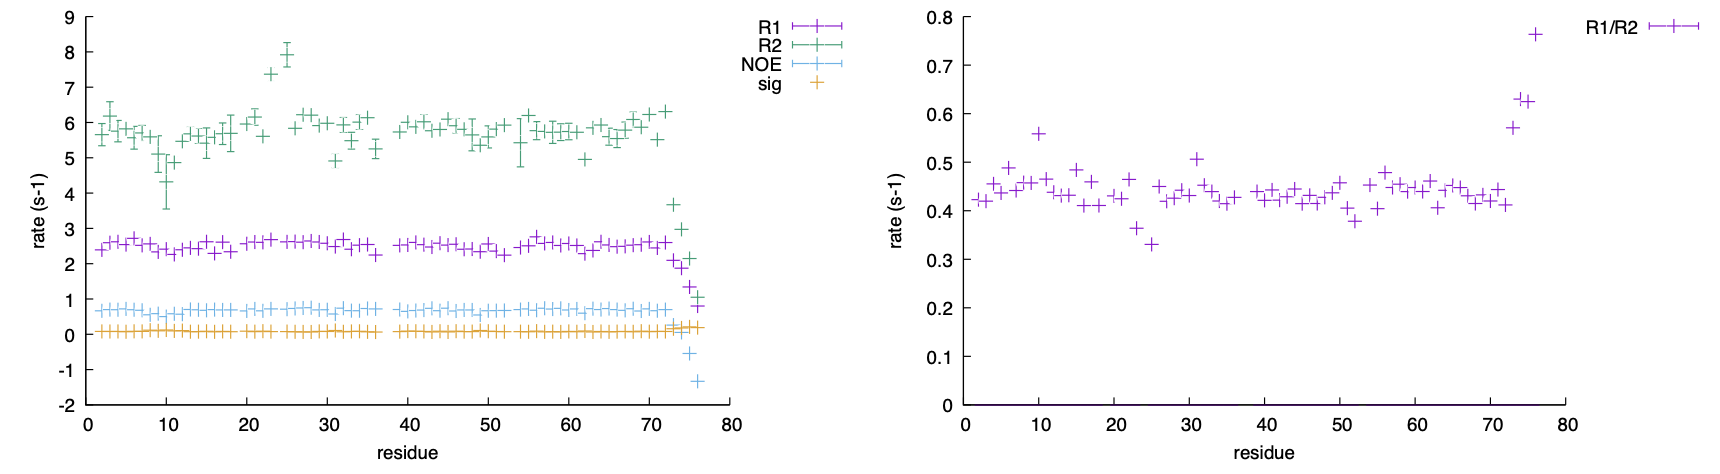
\includegraphics[width=1.0\textwidth]{mathsFigs/ubiquitinData}
  \caption{Ubiquitin relaxation rate, acquired at 500 MHz. As expected, $R_1$ is less than $R_2$, and the NOE is bounded. $\sigma$ is computed from the NOE and $R_1$ using equation \ref{eqNOE}. The $R_2/R_1$ ratio is pretty stable, versus residue.}
\label{Ubifig}
\end{figure}

Lets look at some raw data. We have, amongst other things, Art Palmer's ubiquitin data, acquired at 500 MHz (Figure \ref{Ubifig}) that he's used for various tutorials in how to analyse relaxation data. The $R_1$, $R_2$ and $NOE$ values are shown (Figure \ref{Ubifig}) together with the experimental $R_1/R_2$ ratio, both versus residue. There are 210 measurements here, covering 70 residues. We are going to analyse this data in various ways.

\subsection{Maximally local isotropic tumbling}
\begin{figure}
\center
  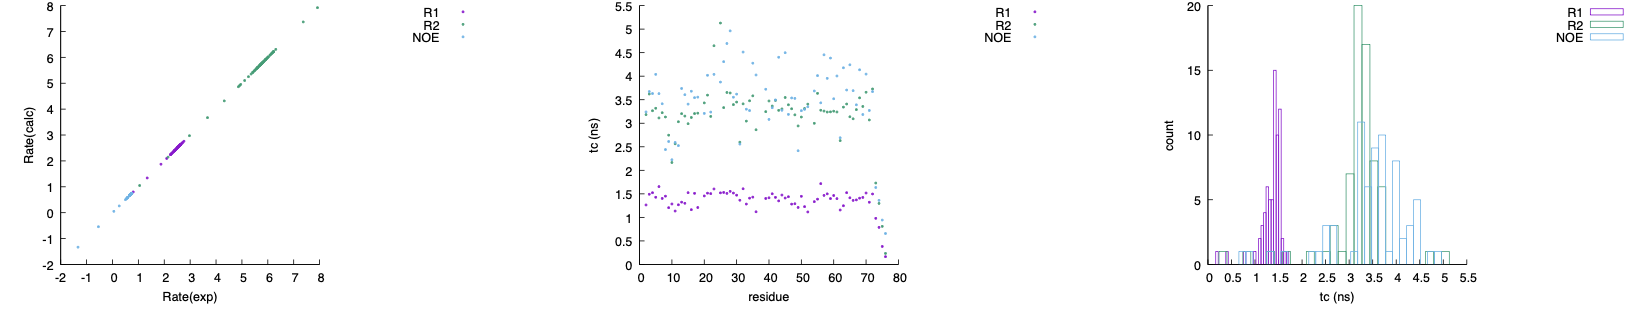
\includegraphics[width=1.0\textwidth]{mathsFigs/RigidCorr}
  \caption{ $R_1$, $R_2$ and NOE rates can be individually associated with a single correlation time, by assuming we have a rigid body isotropic tumbling, and treat reach rate independently. We see that the effective correlation time, at each residue, apparently varies depending on which rate we chose. Typically the effective correlation time from $R_1$ is shorter than that from $R_2$. There are 210 rates shown, which are effectively mapped onto 210 independent correlation times, covering 70 residues. If each residue behaved as a rigid body we would expect to recover the same correlation time from each measured relaxation rate. We do not see this. This means we need to account for local dynamics to properly explain the data, which is also consistent with the correlation times from $R_1$ being shorter than those recovered from $R_2$.}
\label{RigidFig}
\end{figure}

One simple analysis we can do is assume that we have an isotropic rigid body. We can then compute an effective correlation time for each rate (Figure \ref{RigidFig}). This means from 210 measurements we will get 210 correlation times, which do not have to be the same for the three rates measured for a single residue. If ubiquitin behaved truly as a rigid body, then we would expect the same correlation time from each rate and residue. But of course we do not see this. We instead see an average correlation time of 1.35 $\pm$ 0.2 ns from $R_1$, 3.16 $\pm$ 0.7 ns from $R_2$ and 3.5 $\pm$ 0.8 ns from the NOE (see histograms).

The correlation times from $R_1$ are shorter than those from $R_2$ because $R_1$ is dominated by higher frequency transitions. At higher frequencies, the global correlation contribution decreases, but the local correlations stay more constant and so the overall effective correlation time is shortened. Because we see multiple rigid body correlation times per residue, then we know we need need to account for local dynamics. Because there is a 1 to 1 mapping between rate and correlation time, the RMSE here is effectively zero.

\subsection{Isotropic tumbling, one correlation time per residue}

\begin{figure}
\center
  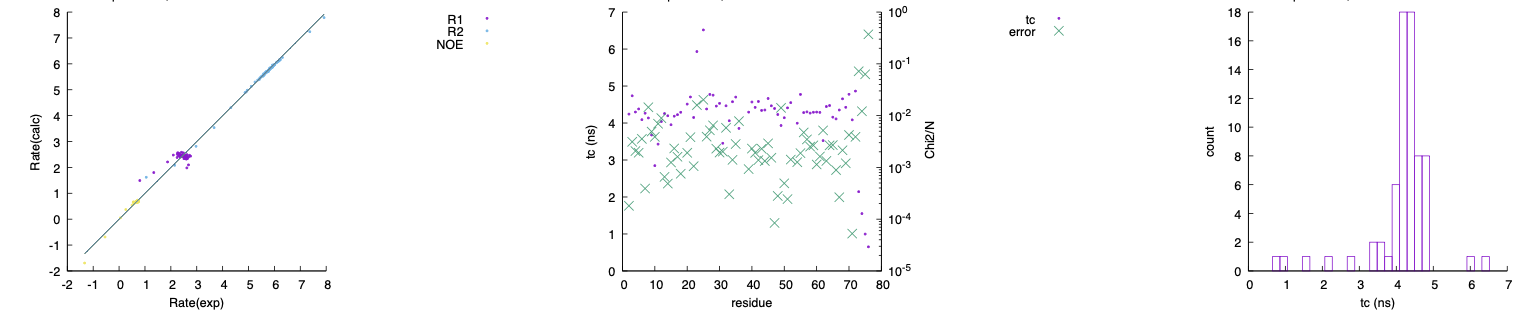
\includegraphics[width=1.0\textwidth]{mathsFigs/IsotropicOnly}
  \caption{Fitting the data using isotropic tumbling but with one correlation time per residue. This means 70 parameters for 210 data points. The average $\tau_c$ is 3.7 $\pm$ 1.4 ns. The reduced $\chi^2$ is 67.5, and the RMSE is 0.14 s$^{-1}$. The local fits are bad only really at the C termini. }
\label{IsoResFig}
\end{figure}

Next, we reduce the parameters by enforcing one correlation time per residue (Figure \ref{IsoResFig}). The fits are not bad, but $R_1$, dominated by local motion, is not well explained. This model has 70 fitting parameters, and gives an RMSE of 0.14. Note that it is unphysical to say that each residue has an independent correlation time.

So we don't get a great fit here and  we are impose a heavy handed approximation. It does perhaps help us see how many correlation times are present.


\subsection{Global isotropic tumbling, one correlation time total}
\begin{figure}
\center
  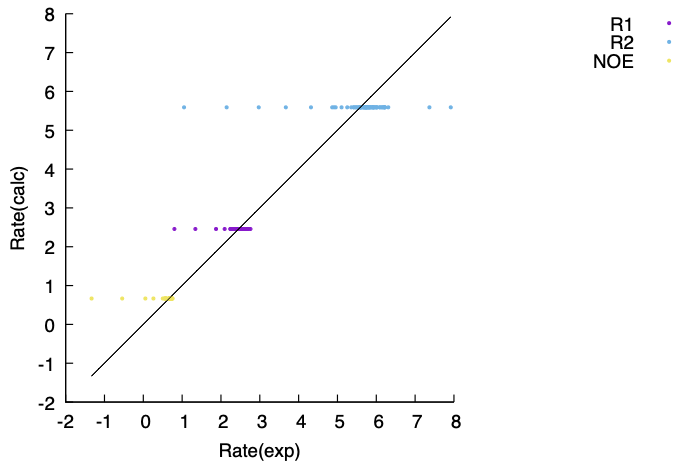
\includegraphics[width=0.5\textwidth]{mathsFigs/IsoGlob}
  \caption{Fitting the data using a single global correlation time. The fitted value is 4.2 ns, the reduced $\chi^2$ is 242, and the RMSE is 0.59 s$^{-1}$. For a single parameter this really isn't bad. But clearly the fit is poor locally. As the model only depends on $\tau_c$, there are only 3 computed relaxation rates, effectively getting re-used for all residues.}
\label{IsoGlobFig}
\end{figure}


Moving the other way, we can ask how well do we do if we fit the entire data with a single correlation time? (Figure \ref{IsoGlobFig}). We do okay, getting a RMSE of 0.6 $s^{-1}$. This model ends up having a single value computed for $R_1$, $R_2$ and $\sigma$, meaning there is no possibility of inter-residue fluctuation. This can be thought of as the `spherical cow' approximation, where we say the protein is a sphere of radius X. The protein does not behave in this way.


\subsection{Global axially symmetric tumbling}

\begin{figure}
  \center
    \includegraphics[width=0.49\textwidth]{mathsFigs/AxialCorr}
  \includegraphics[width=0.49\textwidth]{mathsFigs/Axial}
  \caption{Fitting using axially symmetric global tumbling with alignments coming from a crystal structure. This is shown with $R_1/R_2$ values plotted versus $P_0(\cos\beta^\prime)$, where the angles are computed from the PDB file 1UBQ.pdb. The atomic co-ordinates are extracted, its inertia tensor computed, then aligned with its unique axis and each residues $\beta^\prime$ angle is then derived from the dot product of the NH vector and the unique axis. The reduced $\chi^2$ is 235, with an RMSE of 0.62 s$^{-1}$. The angles that align the diffusion tensor have been fitted, making this a 4 parameter fit. The correlation plot has a non-zero gradient, which suggests anisotropic tumbling. The fitted $\tau_c$ is 4 ns with a shape parameter $\\tau_\parallel/\tau_c$ of 1.18.}
\label{Axialfig}
\end{figure}

A related expansion of this model considers anisotropic tumbling. To work with this, We took a pre-existing structure \verb|1UBQ.pdb|, and added the protons back using openbabel. This piece of software decided to make the NH bond length 0.98 \AA. We then take the structure and move it to its centre of mass. We then compute the inertia tensor and get its three eigenvalues (105001.9, 145651.3 and 159805.9 Da \AA$^2$), so one slightly lower inertia axis, and two larger ones. This means we naively expect ubiquitin to tumble as an oblate spheroid and the axially symmetric model should do quite well. Its radius of gyration and hence correlation times will be proportional to the square root of the moments of interia, and so we expect a ratio of $\sqrt{1.45}=1.2$ for the ratio of the unique, and degenerate correlation times.

We can then compute the dot product of the unique diffusion axis and the NH vectors to obtain the angle $\beta^\prime$ and use this to calculate relaxation rates (and the Legendre polynomial $P_0(\cos\beta^\prime)$). We can see that the ratio $R_1/R_2$ does correlate with $P_0$ (Figure \ref{Axialfig}) suggesting axial diffusion. There are some obvious outliers at the C terminus, but otherwise this is all vaguely linear. Fitting these data to equation \ref{eqp0} allows us to extract the two correlation times $\tau_c$ and $\tau_\parallel$, yielding  4.7 and 5.59 ns respectively. The ratio of these is 1.18 which is very close to the theoretical values.

We can repeat the same optimisation but using the relaxation rates themselves. When we do this, we get a similar result with the correlation plot shown (Figure \ref{Axialfig}). The reduced $\chi^2$ is lower than the isotropic global model at 235, but you still wouldn't call this fit `good'. We can also skip the step involving finding the inertial tensors, and optimise the axis/angle of the diffusion tensor. The data sees a good number of local minima when doing this, so it's a fiddly optimisation that prefers to be started in a good location, which here we can find directly from the structure.

So we cannot well fit the data using models that assume ubiquitin is a rigid body. No surprise really. Onto the next.


\subsection{Incorporating local fluctuations: model free, isotropic}

\begin{figure}
  \center
  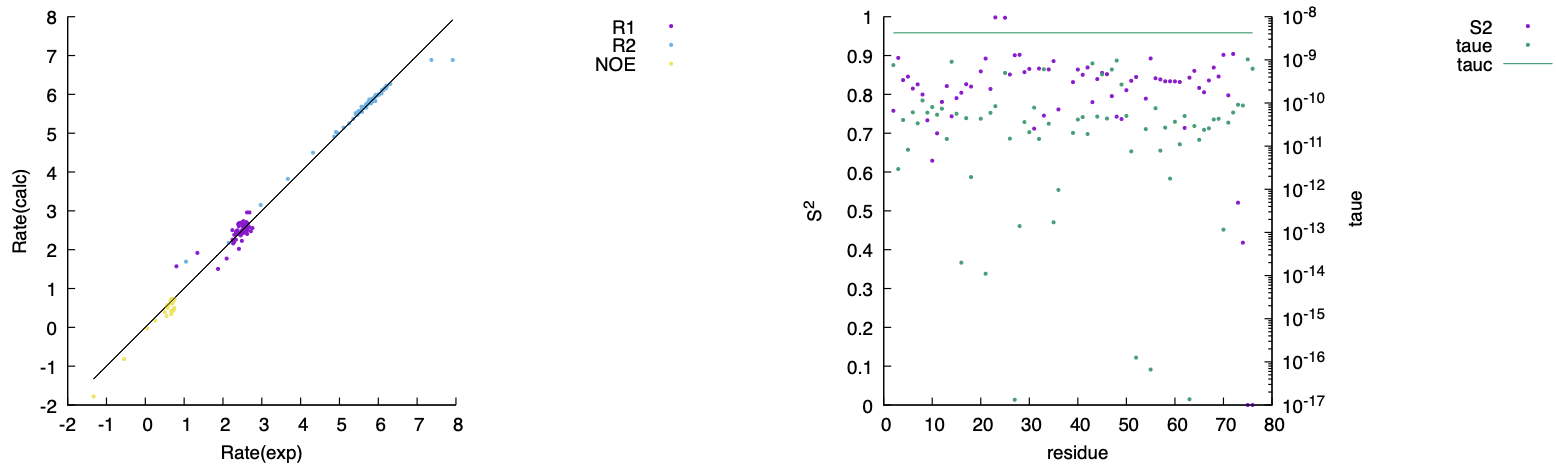
\includegraphics[width=1.0\textwidth]{mathsFigs/IsotropicModelFree}
      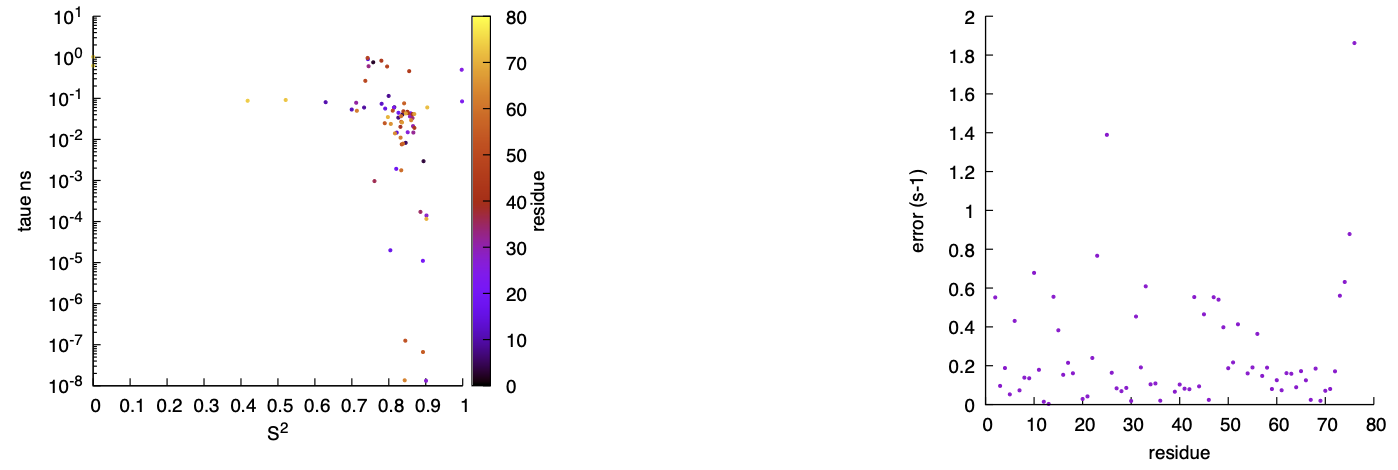
\includegraphics[width=1.0\textwidth]{mathsFigs/IsotropicModelFree2}
    \caption{A model free analysis was performed. The fit gives us a global tumbling time of 4.2 ns, with a range of residue specific order parameters and local correlation times. This is 141 fitting parameters. The average $\chi^2$ is 31.58 and RMSE is 0.16 $s^{-1}$. The order parameter is reasonably constant other than at the $C$ termini where it drops to zero. The local timescale of fluctuations says that most residues experience fluctuations on 20-50 ps. A few residues seem to have an extremely fast local correlation time. Overall, the fit is pretty good but not perfect. Compared to the local residue $\tau_c$ fits, this model is doing a good job of explaining variation in $R_1$. When we look at a plot of $\tau_e$ versus $S^2$ we can see the types of local motion do tend to cluster. Errors in the fit tend to get larger when $\tau_e$ gets large, and exceeds 0.1 ps.
    }
\label{IsoModelFreeFig}
\end{figure}


We need to incorporate the effects of local motion. The obvious place to start is the widely used isotropic model free analysis, where we have a global isotropic tumbling time, and a residue specific order parameter, and local timescale. Applying this gives a reasonable fit (Figure \ref{IsoModelFreeFig}) using 141 parameters. The correlation time that comes out is 4.2 ns and the RMSE has gone down to 0.16 s$^{-1}$. We can see a cluster of residues with an order parameter around 0.85, and a local correlation time between 10-40 ps. This is really emphasised by looking at a plot of $\tau_e$ versus $S^2$, where this cluster is immediately apparent.

We have some residues in the C-termini that are poorly fit - these residues are highly flexible and behave as though they do not experience the global tumbling. Then we have the two residues in the 20s that have unusually high $R_2$ values, which will be because of chemical exchange. So we need some kind of condition that says if the fitted order parameter is very low, close to zero, then global tumbling has no effect whatsoever.

\subsection{Incorporating local fluctuations: model free, axial symmetric}


\begin{figure}
  \center
  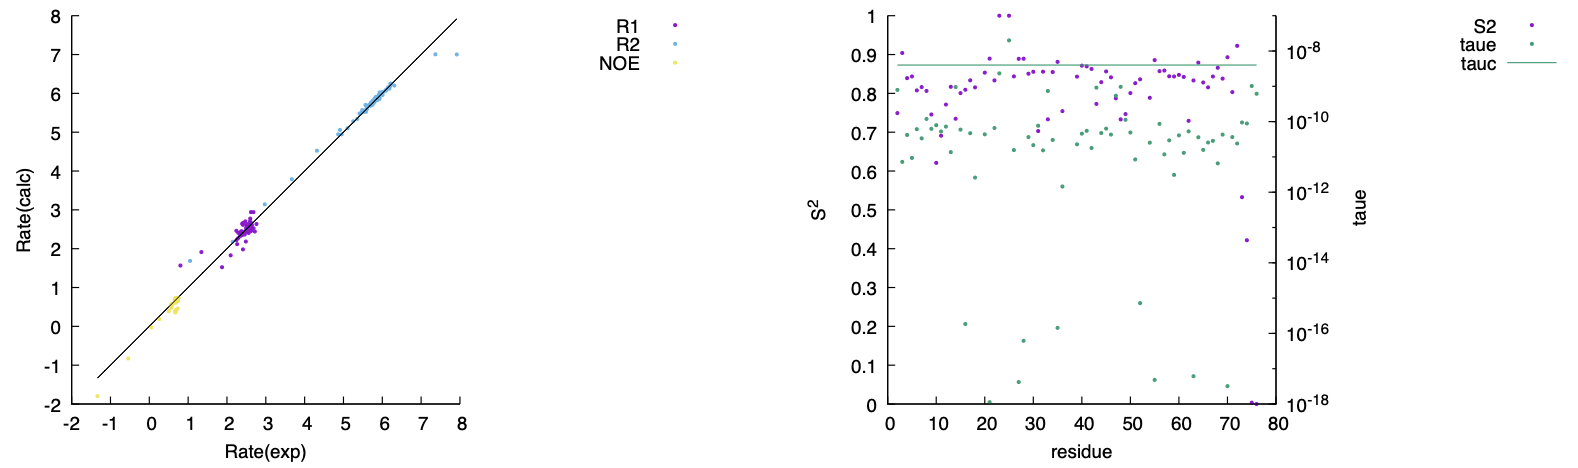
\includegraphics[width=1.0\textwidth]{mathsFigs/AxialModelFree}
      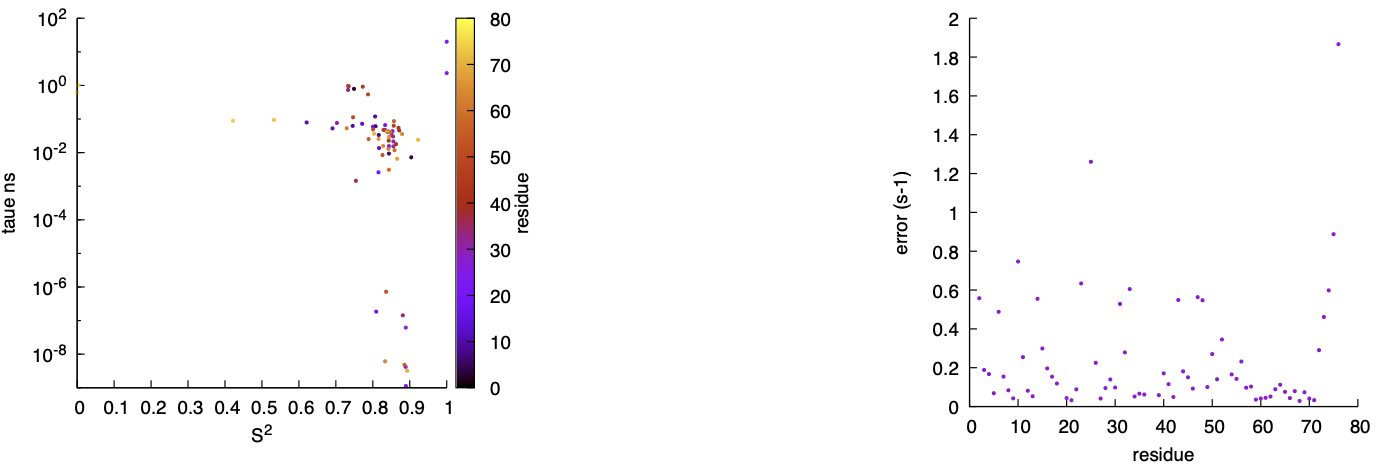
\includegraphics[width=1.0\textwidth]{mathsFigs/AxialModelFree2}
    \caption{A model free analysis was performed using Axial tumbling. The fit gives us a global tumbling time of 4.0 ns and a shape factor of 1.18, with a range of residue specific order parameters and local correlation times. This is 142 fitting parameters. The average $\chi^2$ is 27.89 and RMSE is 0.15 $s^{-1}$. The order parameter is reasonably constant other than at the $C$ termini where it drops to zero. The local timescale of fluctuations says that most residues experience fluctuations on 20-50 ps. A few residues seem to have an extremely fast local correlation time. Overall, the fit is pretty good but not perfect. Compared to the local residue $\tau_c$ fits, this model is doing a good job of explaining variation in $R_1$. The clustering of residues by $\tau_e$ and $S^2$ comes out more strongly here than for isotropic model free. And it is very clear that errors in fitting tend to get large when $\tau_e$ gets large, which seems to apply to residues where the local motion is sufficient to uncouple the residues to global tumbling.
    }
\label{AxialModelFreeFig}
\end{figure}

Moving beyond the isotropic model free model, we can move to the axially symmetric model free fit. Here, we get once again a global tumbling time of 4 ns, a shape factor of 1.18, and an RMSE of 0.15 s$^{-1}$. We have improved! We have some similar problems to the earlier model free approach, that the C terminus is poorly fit and the two exchange broadened peaks are still bad. The clustering however between the order parameter and local timescale is excellent. The axially symmetric model has caused the combinations of $S^2$ and $\tau_e$ to cluster, which feels very sensible.

This is looking pretty great, and is a fertile ground for reduced dimensionality approaches.

\section{Reflections}

Relcalc is a terrific tool for working with this sort of data. We can create any scenario and sets of interactions we want. We can see models that assume ubiquitin is a rigid body fail. But our methods that then admit local dynamics seem to be somewhat unphysical.

In the model free fits, we can see clustering between the order parameter, and the local correlation time. This clustering improves when we incorporate axially symmetric tumbling, indicating that we're on the right track, and this is a fertile space for dimensionality reduction.

There are some areas where the data is simply poorly fit. In the C-terminus, we are degrading the quality of the fit by imposing global tumbling. These actually fit quite well to the very simple single correlation time models. So when residues are `very' flexible and the order parameter is low, the dynamics have become uncoupled from global motion, and the residues are really not experiencing global tumbling. So it doesn't make sense then to impose a single global correlation time. We need to provide the opportunity in fitting for residues to select from more than one option for the global timescale.

In general the fits all get a bit poor when the fitted local timescale is larger than 0.1 ns, so 10\% of global tumbling. This feels intuitive, and suggests that we're simply using the wrong global tumbling time for these residues. This is also indicative of there being enough local motion in say a loop that the dominant mode now is some kind of waving motion, and not overall global rotation.

But: most residues are well accounted for by a combination of a rigid/local timescale combination, where we have $S^2$ about 0.8, a single global tumbling time (that is axially symmetric) with a local fluctuation in the range 20-60 ps. This feels very physical. The rotation of a methyl group has a time constant of about 10 ps, so our jigglings and wigglings here are on this sort of timescale.

We need to implement an appropriate statistical model using dimensionality reduction techniques that allow us to synthesise these motional descriptions.

















%\section{Challenge}

%The problem here is to go from a set of measured relaxation rates, acquired on a per residue basis, to a dynamical model that shows how regions of a protein are moving, and on which timescale.

%The approximation that all spins in the protein are moving at a constant correlation time in a completely rigid body is simply not the case. We can demonstrate this by taking measured relaxation rates, and back calculating their underlying correlation times. If the molecule behaved as a rigid body, the correlation times would all be the same for all rates. Which they are not.

%In the field we routinely then set local timescales and order parameters that are independent of position in the chain. This is also a terrible idea, because it says, among other things, that neighbouring residues do not experience fluctuations on a similar timescale.

%What to do then? We know all sites in the protein are not independent. So it is reasonable to suppose the existence of fluctuations in the molecule occurring over a range of timescales beyond just global tumbling (but it is not reasonable to assume that the timescales are independent at all sites). This is simply because of the topology, that you cannot move one position and keep all the rest constant, while still preserving the fold of the protein. The dynamics must be co-operative, to some extent.

%From analysis of Art Palmers ubiquitin data, we get some immediately interesting features that are not widely discussed. First is that in the bulk of the protein, the correlation time from $R_1$ is lower than the correlation time inferred from $R_2$ and $\mathrm{NOE}$. This implies that the spectral density function is more `peaked' at lower frequencies: that there are additional contributions acting at $J(0)$ that affect $R_2$, that are not affecting $R_1$. This can only be explained by the presence of local dynamics.

%The `effective' correlation time from $R_1$ is hugely sensitive to the inclusion of chemical shift anisotropy, changing by a factor of 2. This interaction is always present, and almost always ignored. This finding is a little bit startling; it means precisely how the dynamics end up being taken out of a complex model depend strongly on the choice of interactions present. Using a tool like RelCalc it's easy to put interactions in/take them out, so we're in a good place to determine how robust our models are with respect to assumptions about the underlying spin physics.

%We have two interesting routes towards a solution here. The first is the one we originally conceived, which is that the acting spectral density comes from a multi-exponential decay of correlation times, where we don't know how many timescales matter. In a very naive case, if we have $3N$ measured relaxation rates, this might suggest we can entertain a maximum of three timescales, and this results in $2N-3$ fitting parameters. As noted by Ollie, the amplitude factors are unlikely to be independent, so we can probably do something clever there to reduce the dimensionality, and perhaps get the number of correlation times a bit higher.

%The other one is newer. We can take all measured relaxation rates, and with our spin physics model associate a correlation time with each. When we do this, we find that for most residues, the correlation times are smallest for $R_1$, middle from $R_2$ and largest from the NOE. It should be possible to sketch out a form of the correlation function that explains this and perhaps allow analytic extraction of some dynamical parameters. This model needs to explain why the correlation function distorts away from a constant rigid body in the way that it does, in the different positions sampled.

%Inspection of the extracted correlation times versus residue number makes it look a lot like there are some principal components. So most cluster around a central value. Can we via clustering or other figure out from these rates a set of unique regimes that inform on co-operative local dynamics?

%In both cases, ultimately we're analysing the data here using methods of dimensionality / parameter reduction. We know the protein is dynamic, and we qualitatively see the effects of dynamics in the raw data. But can we move beyond a picture where we say `part XXX is a bit flappy'?

%We could also take a structural model, ascertain the relative alignment of the NH bond vectors with respect to the inertial frame and look at things via the lens of a known structure. This does feel a bit like cheating though.

%This is an extremely interesting problem. To my knowledge it hasn't been seriously revisited in decades. With software like RelCalc we can easily add in relevant spin physics to try to find a suitable mapping from experimental measurements, to an actual characterisation of the underlying protein dynamics. The problem feels very much like one where we need to reduce the dimensions, and project things onto a more manageable and minimal basis set, which is very much in line with Ollie's approaches.



\end{document}
